\documentclass[conference,compsoc]{IEEEtran}
\usepackage{amsmath}
\usepackage{amssymb}
\usepackage{graphicx}
\usepackage{cite}
\usepackage{url}
\usepackage{booktabs}
\usepackage{multirow}
\usepackage{hyperref}
\hyphenation{op-tical net-works semi-conduc-tor}
\usepackage{titlesec}
% Adjust spacing for sections and subsections
\titlespacing*{\section}{0pt}{1.5ex plus .2ex minus .2ex}{0.7ex plus .2ex}
\titlespacing*{\subsection}{0pt}{1.3ex plus .2ex minus .2ex}{0.5ex plus .2ex}
\titlespacing*{\subsubsection}{0pt}{1.2ex plus .2ex minus .2ex}{0.5ex plus .2ex}

% Remove paragraph indentation and add spacing between paragraphs
\setlength{\parindent}{0pt}
\setlength{\parskip}{0.75em}  % Reduced from 1em to 0.5em


\begin{document}
\title{Graph-Based Game Recommendation System Using Steam User-Item Interactions}
\author{\IEEEauthorblockN{Pablo Deputter}
\IEEEauthorblockA{University of Antwerp\\
Faculty of Science\\
Antwerp, Belgium\\
Email: pablo.deputter@uantwerp.be}
}
\maketitle

\begin{abstract}
This study investigates the effectiveness of graph-based recommendation techniques, particularly Personalized PageRank (PPR), for improving game recommendations on the Steam platform. We compare PPR and its variants (Multi-Alpha PPR and TwoPhase PPR) against traditional recommendation algorithms using a dataset of user-game interactions. Our evaluation focuses on strong generalization with unseen users and employs metrics including NDCG@20 and Recall@20. The study analyzes how different parameters affect recommendation quality and explores the trade-offs between model complexity and performance. We examine whether more complex PPR variants provide meaningful improvements over the basic implementation and investigate the relative importance of personalization versus popularity-based signals. Our findings provide insights into the practical implementation of graph-based recommendation systems in the gaming domain and suggest directions for future research in game recommendation systems.
\end{abstract}

\section{Introduction}
Recommender systems are crucial for navigating the vast catalogs of modern online platforms. In the gaming industry, particularly on Steam, players face challenges finding games that match their preferences among thousands of titles. This research investigates how graph-based recommendation techniques, specifically Personalized PageRank (PPR), can improve game recommendation accuracy on the Steam platform.

The study focuses on comparing PPR's effectiveness against traditional recommendation algorithms, examining both accuracy and computational requirements. We analyze how different PPR parameters affect recommendation quality and explore variants like MultiAlpha PPR and TwoPhase PPR. Our hypothesis suggests that PPR will outperform conventional methods in accuracy due to its ability to capture complex user-item relationships, albeit with higher computational costs.

\section{Background and Related Work}
Modern online platforms rely heavily on recommender systems to help users discover relevant content among vast options. While traditional approaches focused on direct user-item interactions, contemporary systems leverage complex relationships between users and items to generate more sophisticated recommendations.

\subsection{Collaborative Filtering}
Collaborative filtering (CF) predicts user preferences by analyzing patterns in user-item interactions across a community of users. Traditional CF approaches include memory-based methods using similarity metrics between users or items, and model-based techniques like matrix factorization. However, CF methods often struggle with data sparsity and the cold-start problem for new users~\cite{1707.07435}, motivating the development of alternative approaches.

\subsection{Graph-Based Recommender Systems}
Graph-based methods offer an alternative to CF, representing user-item interactions as a graph structure~\cite{1812.08434}. In this approach, users and items are represented as nodes, and interactions as edges. Graph algorithms can then be applied to this network to make recommendations by considering the connections within the graph. This approach has the advantage of using the inherent relationships between users and items to make recommendations~\cite{1707.07435}.

\subsubsection{Personalized PageRank (PPR)}
PPR is a graph-based algorithm derived from the original PageRank algorithm~\cite{ilprints422}, which was designed for ranking webpages. It addresses the limitations of traditional PageRank in the context of recommendation by introducing a personalization vector, which biases the random walk on the graph~\cite{Haveliwala2002}. This vector tailors the random walk according to a specific user's history, thereby generating personalized recommendations that align with their preferences.

The algorithm simulates a random walker, starting from a user node, exploring the graph through edges, and assessing the relevance of item nodes based on the frequency of visits. The probability of the random walker jumping to a specific item is proportional to the weight of the edge, allowing for exploration of the graph. The importance of this item is then determined by the probability of the random walk visiting it. The iterative nature of the algorithm is represented mathematically as:

\begin{equation}
    r^{(t+1)} = \alpha A r^{(t)} + (1-\alpha)v
\end{equation}

\noindent where $r^{(t)}$ represents the relevance score vector at iteration $t$, $A$ is the transition probability matrix derived from the graph's adjacency, $\alpha$ is the damping factor controlling the random walk's behavior, and $v$ is the personalization vector.\footnote{In our formulation, $\alpha$ represents the probability of following graph edges, whereas in the traditional literature, $\alpha$ typically represents the complementary restart probability.} The damping factor $\alpha$ controls the balance between exploration and exploitation, with higher values favoring edges from the graph, and smaller values favoring items from the user's history. The personalization vector $v$ directly encodes user preferences, typically being a normalized vector of the user's item interactions.

\subsubsection{Graph Neural Networks (GNNs)}
Graph Neural Networks (GNNs) have been proposed for learning node representations in graphs~\cite{1812.08434}. In recommender systems, GNNs iteratively aggregate information from the neighborhood of each node, generating embeddings that are used to predict interactions. While models like LightGCN~\cite{2002.02126} simplifies traditional GCNs, GNNs have a major limitation for this project. They depend on pre-learned node embeddings, making them unsuitable for this project as we aim for strong generalization with unseen users, and GNNs also have higher computational resource needs~\cite{1707.07435}.

\section{Methodology}
This section outlines our approach to evaluating personalized game recommendations using the Steam dataset. We describe our data preprocessing methodology, algorithmic approaches ranging from basic baselines to advanced graph-based methods, and our evaluation framework that emphasizes strong generalization through testing on unseen users and items. Our methodology ensures findings reflect real-world applicability while maintaining reproducibility.

\subsection{Dataset}
The Steam dataset, initially introduced by Kang and McAuley \cite{1808.09781} and later used in other studies \cite{Wan2018,Pathak2017}, forms the basis of our analysis. It contains $2,293,985$ interaction records between $54,315$ unique users and $8,368$ unique games. A key characteristic of this dataset is the right-skewed distribution of playtime, which results in high playtime outliers. This skew is evident when observing the original distribution of playtime, as well as user activity and item popularity, with long-tailed distributions where the majority of values are concentrated at lower ranges, and a few extreme values are present. To mitigate the effect of these outliers and enhance the visibility of lower-end values, a log-transformation is applied, which is crucial for the model as extreme values would negatively impact model performance.

\subsubsection{Strong Generalization}
We evaluate the models under a strong generalization setting where the test set contains only users and items not seen during training. This ensures a more robust assessment of the model's capacity to generalize to new, unseen data, an essential condition for real-world applicability.

\subsection{Data Preprocessing}
This section details the data preprocessing steps used to prepare the dataset for our experiments. The main goals of this stage are to manage the size of the dataset, create realistic train/validation/test splits and properly handle the playtime values.

\subsubsection{Data Sampling}
Given the computational constraints of processing large-scale interaction data, we implemented a stratified sampling approach that preserves the underlying distribution characteristics of the full dataset. Users are partitioned into five quantile-based bins based on their interaction frequency, ensuring representation across different activity levels. The number of users sampled from each bin is calculated as:
\begin{equation}
n_{bin} = n_{users} \cdot \frac{|bin_{users}|}{|users|}
\end{equation}
where $n_{bin}$ represents the number of users sampled from each activity bin, $n_{users}$ is the total desired sample size, and $|bin_{users}|$ is the number of users in that particular bin. This stratification is crucial as it maintains the heterogeneity of user behaviors present in the original dataset, particularly important for capturing both casual and power users.

\subsubsection{Data Split Strategy}
Our data splitting methodology creates realistic evaluation scenarios through a two-phase process that preserves distribution similarity across splits.
\paragraph{\textbf{Train-Validation Split}}
The dataset is split 80/20 using a similarity-based selection mechanism. Users are scored based on their similarity to the test set distribution:
\begin{equation}
score_{user} = 0.4 \cdot score_a + 0.4 \cdot score_i + 0.2 \cdot score_p
\end{equation}
where $score_a$, $score_i$, and $score_p$ represent activity, item preference, and playtime similarity scores respectively. Selection probabilities are computed using softmax:
\begin{equation}
P(user) = \frac{e^{score}}{\sum_i e^{score_i}}
\end{equation}
\paragraph{\textbf{Fold-based Validation Split}}
The validation set is divided into fold-in and fold-out sets, where the number of items per user follows the test set distribution:
\begin{equation}
n_{items} \sim \mathcal{N}(\mu_{test\_items}, \sigma_{test\_items})
\end{equation}
Items are selected using a weighted score of popularity and engagement:
\begin{equation}
score_{item} = 0.7 \cdot score_{popularity} + 0.3 \cdot score_{playtime}
\end{equation}
\subsubsection{Empirical Validation}
Figure~\ref{fig:split_validation} demonstrates the effectiveness of our splitting strategy through distribution analysis across four dimensions. The Jensen-Shannon divergence between validation and test sets shows strong alignment (activity: $0.138$, popularity: $0.138$, playtime: $0.021$), with particularly strong playtime pattern preservation (KL divergence: $0.0015$). The fold-based split maintains a balanced $0.90$ ratio between training history and future interactions, creating realistic evaluation conditions while preventing data leakage.
\begin{figure}[h]
\centering
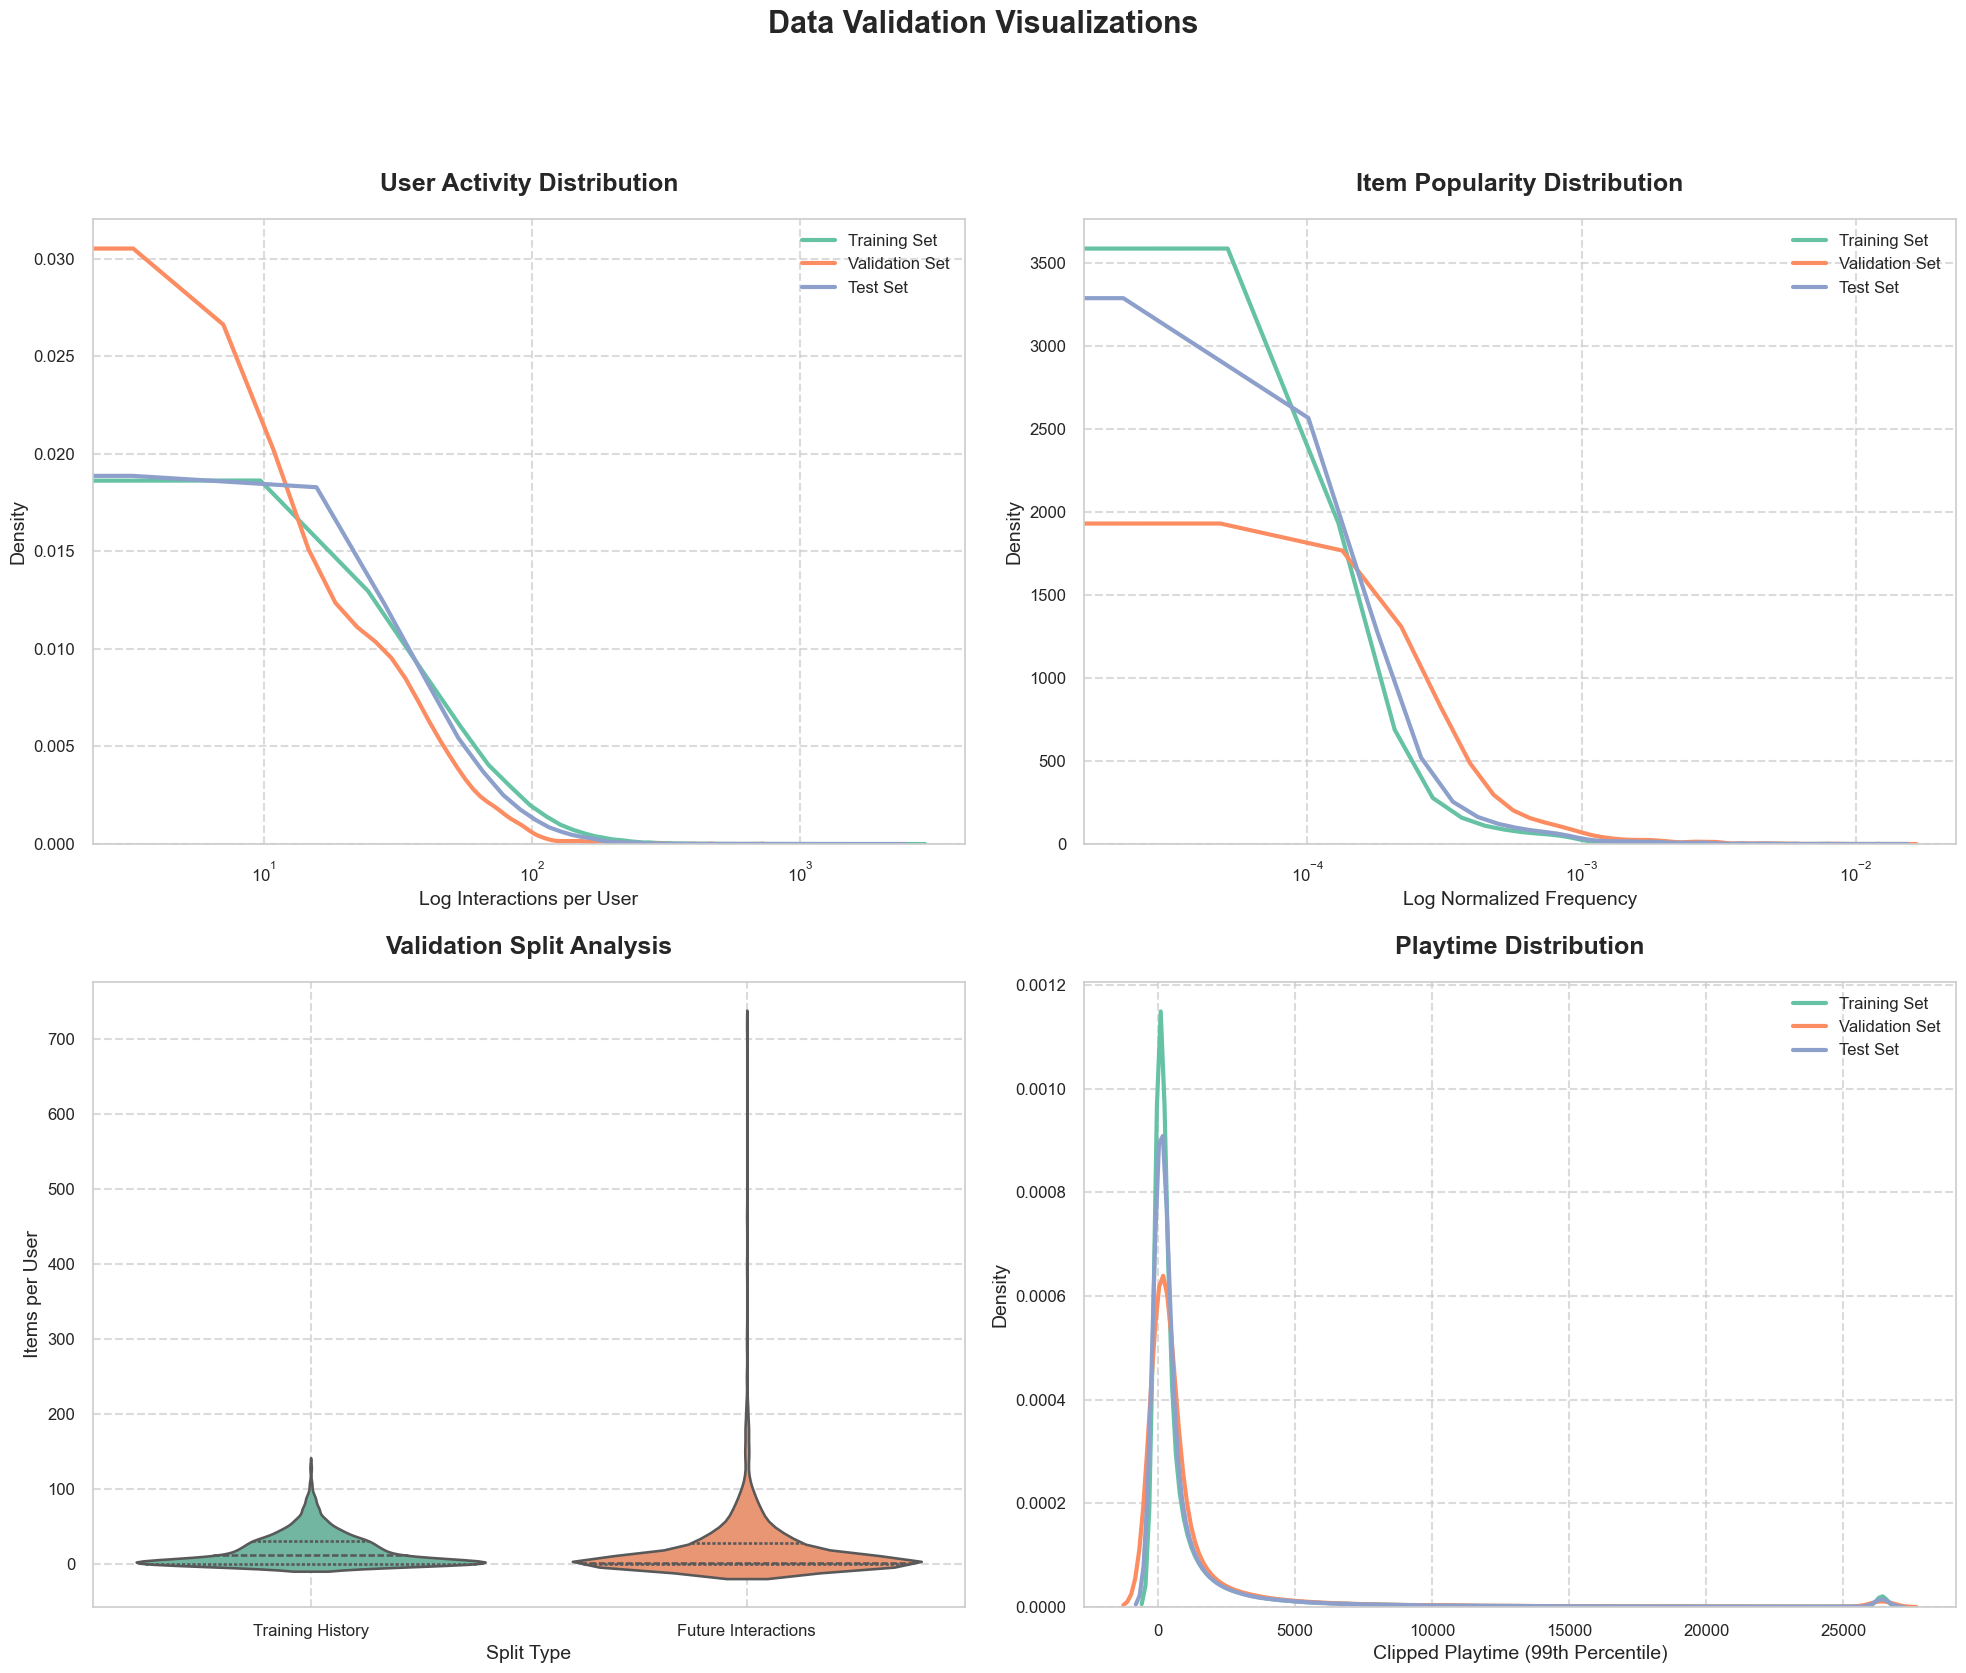
\includegraphics[width=0.5\textwidth]{images/split_validation.png}
\caption{Validation of data split representativeness showing (a) user activity distribution, demonstrating preserved interaction patterns across splits; (b) item popularity distribution, indicating maintained popularity dynamics; (c) validation split analysis, showing balanced fold-in/fold-out proportions; and (d) playtime distribution, confirming consistent engagement patterns.}
\label{fig:split_validation}
\end{figure}
The results confirm our splitting methodology successfully preserves user activity patterns, maintains item popularity distributions, ensures consistent engagement patterns, and creates realistic evaluation scenarios through balanced splitting.

\subsubsection{Playtime Transformation}
To mitigate the effect of outliers, we apply a logarithmic transformation to user playtime:
    \begin{equation}
        x' = \log(1 + x)
    \end{equation}
where $x$ represents the original playtime. This transformation reduces the skew of the data by compressing high values, enhancing the contribution of smaller values. After this transformation, min-max scaling is used to scale the transformed values between 0 and 1.

\subsubsection{Relative Scaling}
Playtime data is also scaled relative to each user's average playtime. This approach ensures that the model gives more weight to interactions that are relevant to a specific user's historical playtime patterns.
\subsection{Algorithms}
This section details the different algorithms that are used, ranging from basic baseline techniques to the more advanced graph-based methods.

\subsubsection{Baselines}
We use several baselines to establish a comparison point for our model performance:
\begin{itemize}
    \item \textbf{Random Recommendations}: Serves as a low-end baseline by recommending items randomly. This approach will show the performance of random chance and will serve as a baseline.
    \item \textbf{Popularity}: Recommends the most popular items based on the number of interactions, providing a basic approach for recommendations when no personalization is used.
    \item \textbf{User-kNN}: Recommends items based on the preferences of similar users using cosine similarity.
    \item \textbf{Item-kNN}: Recommends items similar to those the user has interacted with previously, based on cosine similarity between items.
\end{itemize}
These baselines represent common recommendation strategies, and offer a comparison point for more advanced algorithms that take personalization into account.

\subsubsection{Personalized PageRank (PPR)}
PPR is a graph-based algorithm that models user-item interactions as a bipartite graph, where users and items are represented as nodes, and interactions as weighted edges. PPR simulates a random walker navigating this graph, biased toward items based on a user's history. This simulates how a users preferences are propagated using the information encoded in the graph.  The iterative nature of PPR relies on a power iteration process, repeatedly updating the relevance score vector \(r\) until it meets a convergence criteria or until the \(num\_iterations\) parameter is met.

The transition probabilities are derived from the user-item interaction matrix (\(W\)), which contains raw interaction values like playtime. The matrix \(W\) is transformed into \(W'\), by log transformation and normalization or relative scaling as seen earlier, which are then used to calculate the transition probabilities.  The transition probability matrix \(A\) is calculated as \(P_{IU} \cdot P_{UI}\), reflecting a two-step random walk from item to user and back to item. The user-item transition probability matrix (\(P_{UI}\)) is calculated from the transformed user-item interaction matrix \(W'\), with each row normalized:

\begin{equation}
    P_{UI}(j, i) = \frac{w'_{ji}}{\sum_{k}w'_{ki}}
\end{equation}

where $w'_{ji}$ represents the interaction strength between user $i$ and item $j$ in $W'$. The item-user transition probability matrix ($P_{IU}$) is obtained by transposing the normalized $P_{UI}$ matrix. Since transposition changes columns to rows, we need to ensure each row still sums to 1, leading to:

\begin{equation}
    P_{IU}(i, j) = \frac{w'_{ij}}{\sum_{k}w'_{ik}}
\end{equation}

The user-item graph is visualized in Figure \ref{fig:transition_network}, where edge thicknesses are based on transition probabilities.

The iterative update formula for PPR is:
\begin{equation}
    r^{(t+1)} = \alpha A r^{(t)} + (1-\alpha)v
\end{equation}
where:
\begin{itemize}
    \item \(r^{(t)}\) is the relevance score vector for all items at iteration \(t\), representing the probability of the random walk ending at a specific item given the current random walk.
    \item \(\alpha\) is the damping factor, with a range between 0 and 1, controlling the balance between exploration and exploitation of the random walk, which is biased by the personalization vector.
   \item \(v\) is the personalization vector. This vector is based on user's historical interactions, and is initialized using a log-transformed version of the raw interactions. The transformed playtime vector \(t_{log}\) is calculated as:
        \begin{equation}
            t_{log} = log(1+t)
        \end{equation}
where \(t\) is the original playtime vector. The personalization vector is then set using:
     \begin{equation}
     v_j = \begin{cases}
           t_{norm,j} & \text{ if item j is in history} \\
           0 & \text{ otherwise}
       \end{cases}
    \end{equation}
 where $t_{norm,j}$ is a normalized version of the user's historical interaction for item $j$. This ensures seed items influence the random walk equally.
\end{itemize}
\begin{figure}[!ht]
    \centering
    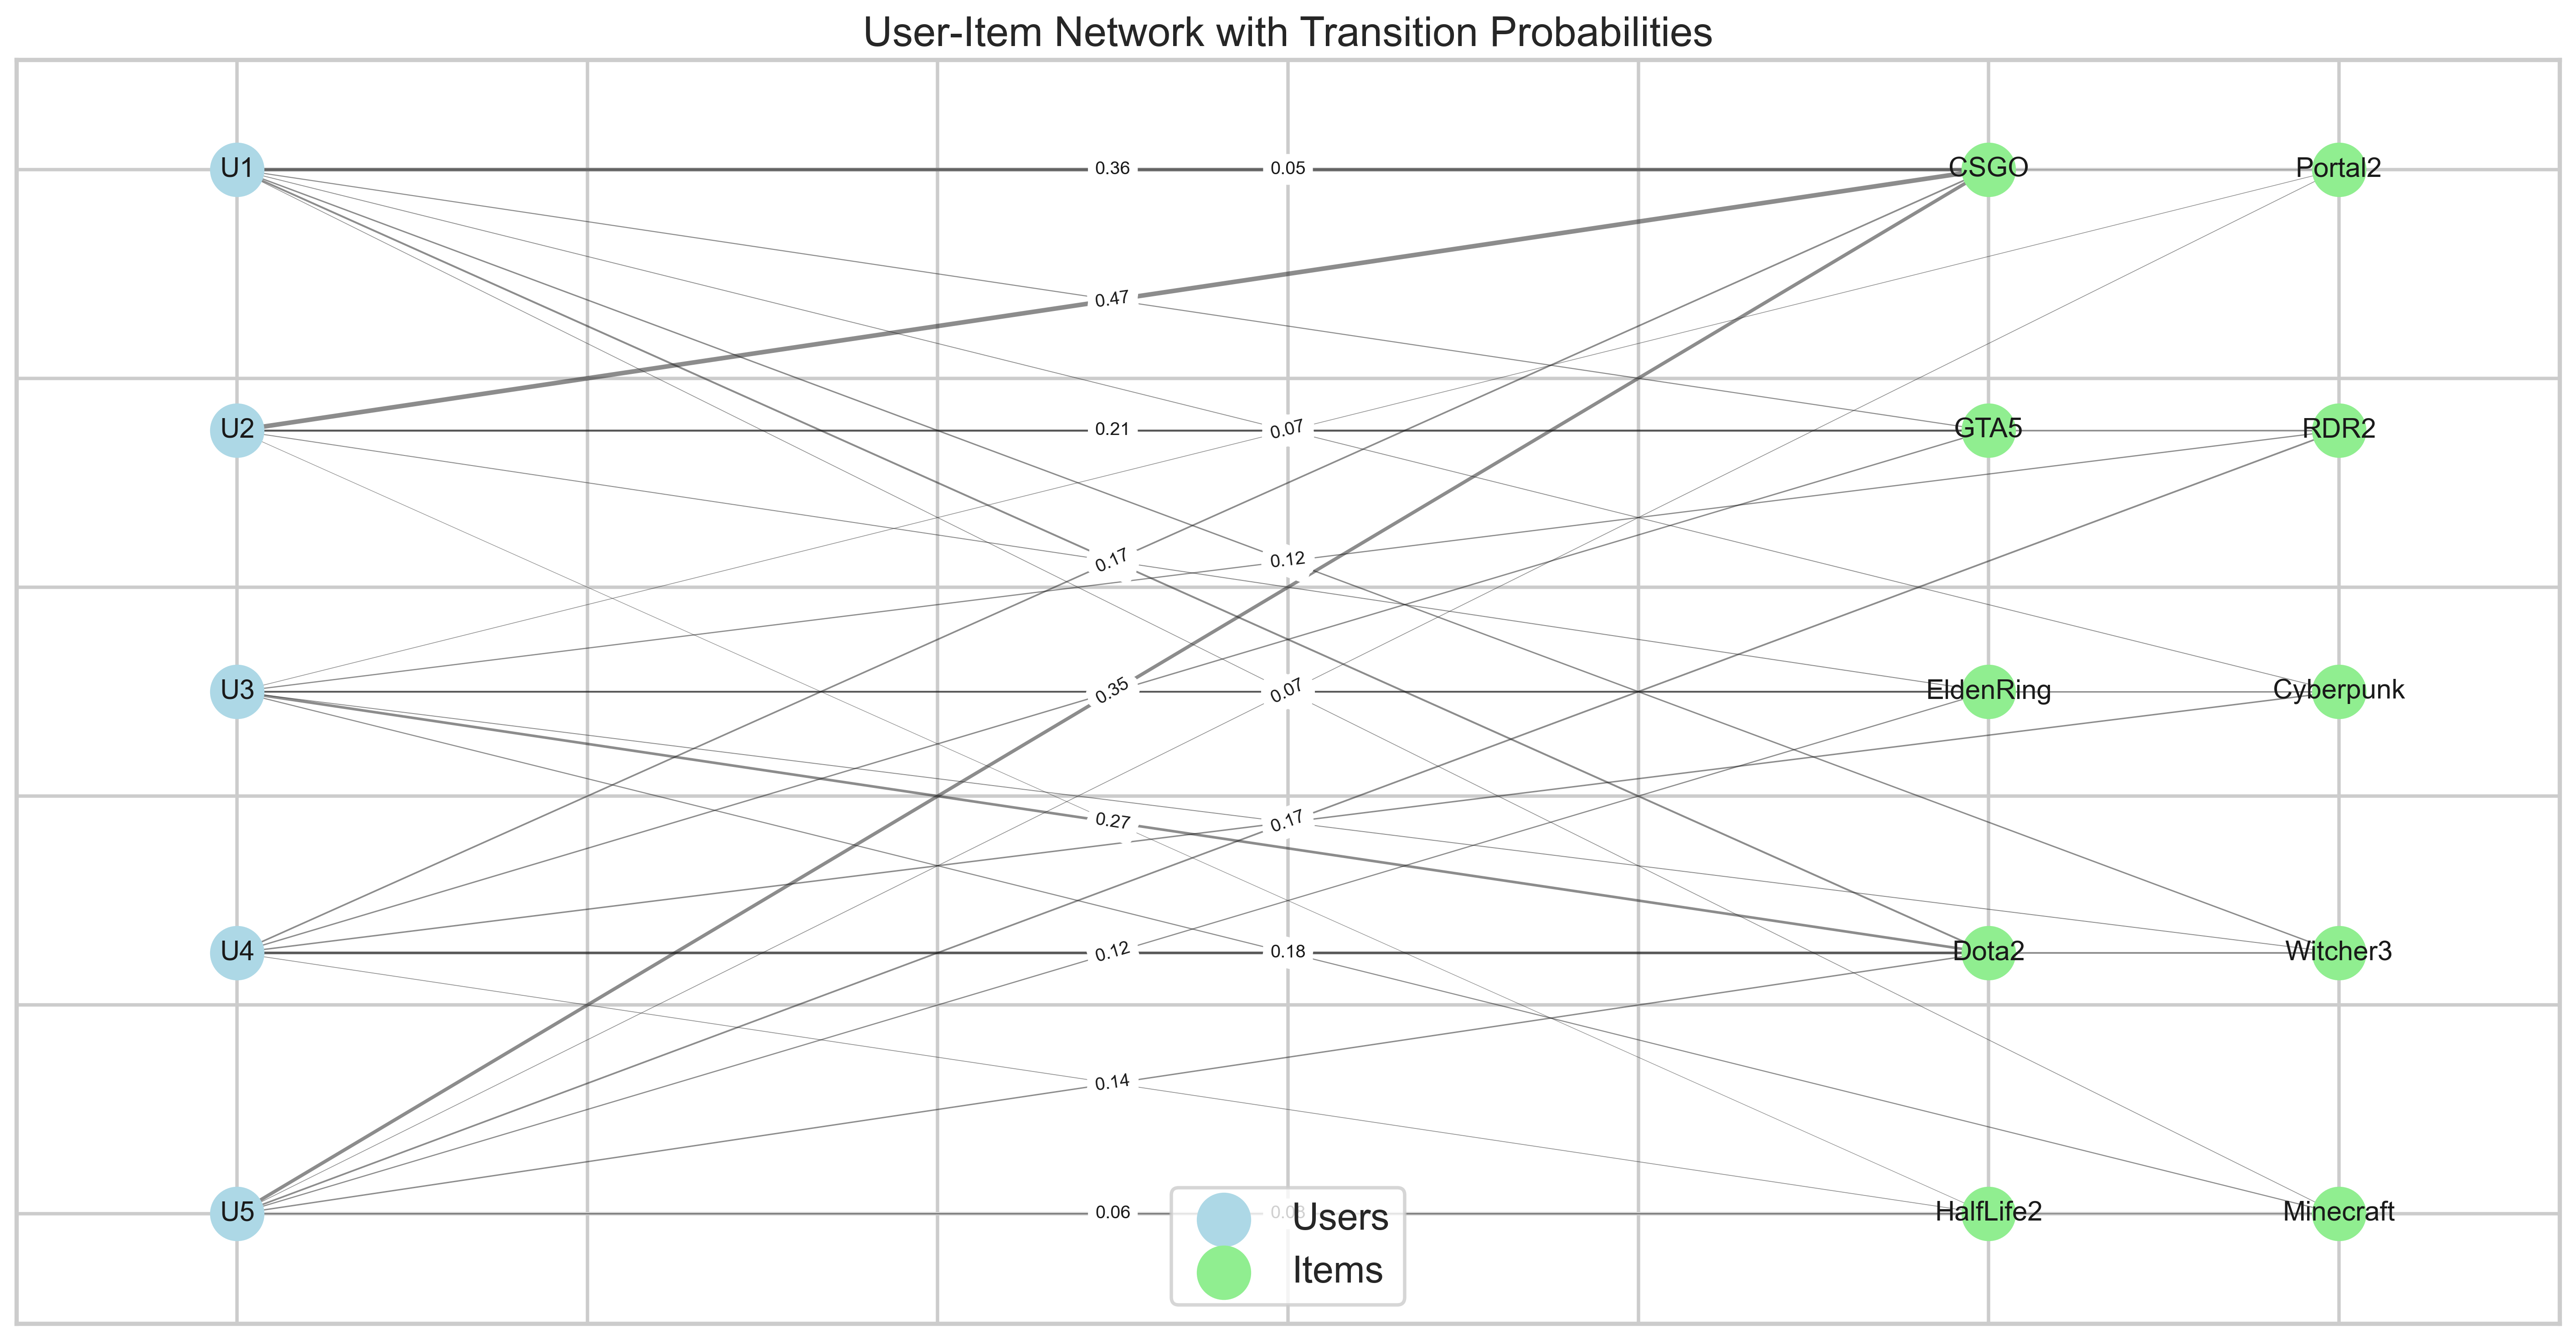
\includegraphics[width=\linewidth]{images/transition_network_fixed.png}
    \caption{Example user-item interaction network as a bipartite graph, where the edge thickness represents the transition probabilities.}
    \label{fig:transition_network}
\end{figure}

After calculating the PPR scores, historical item interactions are masked out to ensure that the recommendations do not include items the user has already interacted with. The final recommendation scores are calculated using:
    \begin{equation}
        score_j = (1 - w(h)) \cdot r_j + w(h) \cdot pop_j
    \end{equation}
where \(r_j\) is the PPR score of item \(j\), and \(pop_j\) is a popularity score of item \(j\), which provides a fallback for users with short interaction histories. This score is calculated by summing the transformed interactions of an item across all users using:
    \begin{equation}
        pop_j = \sum_{i=1}^{n}w'_{ij}
    \end{equation}
where \(w'_{ij}\) is the interaction strength for item \(j\) of a total number of users \(n\), derived from the transformed user-item interaction matrix \(W'\). The adaptive popularity weight \(w(h)\) balances item popularity and personalized scores:
    \begin{equation}
        w(h) = \begin{cases}
        0.9 & \text{ if h = 0 (no history)} \\
        min(0.5,w_b + (5-h) \cdot 0.1) &  \text{ if } 1 \leq h \leq 5 \\
       w_b & \text{ if } h > 5
        \end{cases}
    \end{equation}
where \(h\) represents the length of a user’s interaction history, and \(w_b\)  is a base popularity weight parameter. This dynamic weighting ensures that the model has a proper balance between popularity and personalization. Finally, the top N items with highest scores are recommended.

\subsubsection{PPR Variants}

\paragraph{\textbf{Multi-Alpha PPR}}
This variant of PPR leverages multiple alpha values to create a more robust representation of user preferences, allowing it to capture both broad and specific interests. Multiple PPR scores are calculated for each alpha, which are then combined using weights:

        \begin{equation}
        r_{final} = \sum_{i=1}^n w_i \cdot r^{(i)}
        \end{equation}
     where \(r^{(i)}\) are the PPR vectors obtained using different alpha values \(i\), and \(w_i\) are the corresponding weights that determine the level of influence of each vector, constrained to sum up to 1 to normalize the final result. This design is made to create a stronger view of the graph, as multiple random walks, capturing different depths and biases, are calculated and combined.

\paragraph{\textbf{Two-Phase PPR}}
This method splits the PPR calculation into two distinct phases, combining exploration and exploitation for more balanced recommendations. The first phase is a broad exploration using a higher \(\alpha_1\) to discover a wide set of potential recommendations. Then, the top $k$ most relevant items from the first phase are used to calculate a new personalization vector. Finally, in the second phase, a second PPR calculation is performed using a lower \(\alpha_2\), providing more focused results based on the most relevant items from phase one. This two-phase design allows for a mix of exploration to identify a range of candidates, and exploitation to fine-tune the final recommendations.

\subsection{Evaluation Metrics}
Recommendation performance is assessed using two key metrics that evaluate recommendation quality:

\paragraph{\textbf{NDCG@20}}
NDCG measures ranking quality of the top-20 recommendations. It emphasizes the importance of having relevant items appear at the top of the recommendation list. A perfect NDCG score indicates that the most relevant items are positioned at the highest ranks.

\paragraph{\textbf{Recall@20}}
Measures the proportion of all possible relevant items that appear within the top-20 recommendations. This metric focuses on the system's ability to find relevant items, regardless of their exact position within the top 20.

Additionally, computational efficiency is evaluated by tracking total execution time, which includes both training and inference phases.

\subsection{Experimentation}
This section details the experimental setup, explaining the evaluation approach and the parameter optimization process.

\subsubsection{Offline Evaluation}
Given the scale and computational demands, the performance of our models is first evaluated offline using a local evaluation setup. This approach is structured as follows:
\begin{itemize}
    \item \textbf{Sampling}: A subset of the data is sampled from the training set while maintaining the original user activity distribution as explained in  the "Data Preprocessing" section. This ensures that the sampled data set represents the characteristics of the complete training data, to better understand the model performance.
\item \textbf{Cross-Validation}: We employ nested 3-fold cross-validation, dividing the dataset into train and validation sets. The validation set is further split into fold-in (for generating recommendations) and fold-out (ground truth) sets. Multiple random seeds are used across folds to ensure robust evaluation and reduce selection bias.
\item \textbf{Trials}: Each evaluation is repeated three times with different random seeds (seed, seed+1, seed+2) to ensure reproducibility and assess model stability across varying data splits.
    \item \textbf{Metrics}: During each fold, the models are evaluated using NDCG@20 and Recall@20, to assess ranking quality and the ability to recall all relevant items, respectively.
\end{itemize}
 The evaluation process outputs average values across the different trials, with standard deviations as measures of the robustness of results.

\subsubsection{Hyperparameter Tuning}
We employ Bayesian optimization to find optimal hyperparameters, using a Gaussian Process to guide the search based on past evaluations. The optimization maximizes a weighted combined score:
\begin{equation}
    \text{Combined Score} = 0.85 \cdot \text{NDCG@20} + 0.15 \cdot \text{Recall@20}
\end{equation}
This emphasizes ranking quality while considering retrieval performance. The hyperparameter exploration process is initiated using a base seed to ensure reproducibility across optimization runs.

\subsubsection{Online Evaluation}
To assess the performance of our optimized models on the unseen test set, we generate recommendations. This is done by training the models on the entire training dataset and then evaluating its performance on the completely held-out test set, that contains entirely new users that the model did not see during training. The total time it takes for the full training and prediction procedure is tracked.

\section{Results}
This section presents the experimental results of the different recommendation algorithms. We start with the baselines, followed by PPR and its variants. All results were obtained using the earlier described evaluation setup.

\subsection{Baseline Results}
Table \ref{tab:baseline_results} shows the performance of these baselines. Random recommendations perform poorly, demonstrating the need for capturing user-item relationships. Item-KNN stands out as the best performing baseline, showing that similar items tend to have strong relations. The popularity model performs reasonably well, indicating many items are universally liked. User-KNN shows identical performance to popularity because it falls back to popularity-based recommendations for users not seen during training, highlighting limitations in capturing user similarity alone.
\begin{table}[!ht]
    \centering
    \caption{Online Baseline Performance}
    \label{tab:baseline_results}
    \begin{tabular}{@{}lccccc@{}}
    \toprule
    \textbf{Algorithm} & \textbf{SubID} & \textbf{NDCG@20} & \textbf{Recall@20} & \textbf{Time (s)} \\
    \midrule
    Random  & 188908 & 0.002 & 0.003 & 8.32 \\
    Popularity & 188941 & 0.208 & 0.285 & 1.63 \\
    User-kNN & 188910 & 0.208 & 0.285 & 51.30 \\
    Item-kNN & 188503 & 0.320 & 0.352 & 5.65 \\
    \bottomrule
    \end{tabular}
\end{table}


\subsection{Personalized PageRank (PPR) Results}
After hyperparameter optimization, the PPR model achieves a good performance, outperforming most baselines, with a similar performance as Item-KNN. Table \ref{tab:ppr_results} shows the optimized parameters, the offline metrics and the execution times of the PPR method. The very low values for the optimized alpha (0.023) and the popularity weight (0.033) indicate a very strong reliance of the model on the personalization vector rather than exploration using the random walk, and that global item popularity adds less value to the recommendations. The moderate number of iterations (93) also highlights that the power iteration process converges rather quickly, and that further computation will lead to diminishing returns. The parameter optimization process consistently found the log transformation achieved a better performance than relative scaling.

\begin{table}[!ht]
\centering
\caption{PPR Optimized Parameters and Results}
    \label{tab:ppr_results}
\begin{tabular}{lc}
\toprule
\textbf{Parameter} & \textbf{Value} \\
\midrule
Alpha & 0.023 \\
Popularity Weight & 0.033 \\
Iterations & 93 \\
Offline NDCG@20 & 0.3449\\
Offline Recall@20 & 0.4172\\
Execution Time (s) CPU / GPU & 280 / 30-45 \\
\bottomrule
\end{tabular}
\end{table}
The figures \ref{fig:ppr_alpha},  \ref{fig:ppr_popularity} and \ref{fig:ppr_iterations} show the hyperparameter optimization of alpha, popularity weight and number of iterations respectively, and how they relate to the weighted score, as well as NDCG and Recall. The plots for alpha and popularity weight show that the best results are in areas where both parameters have low values, highlighting that more personalized approaches work best for this dataset. Also, in the num\_iterations plot, it is visible that performance plateaus after a certain threshold, which justifies the choice for 93 iterations.
\begin{figure}[!ht]
    \centering
    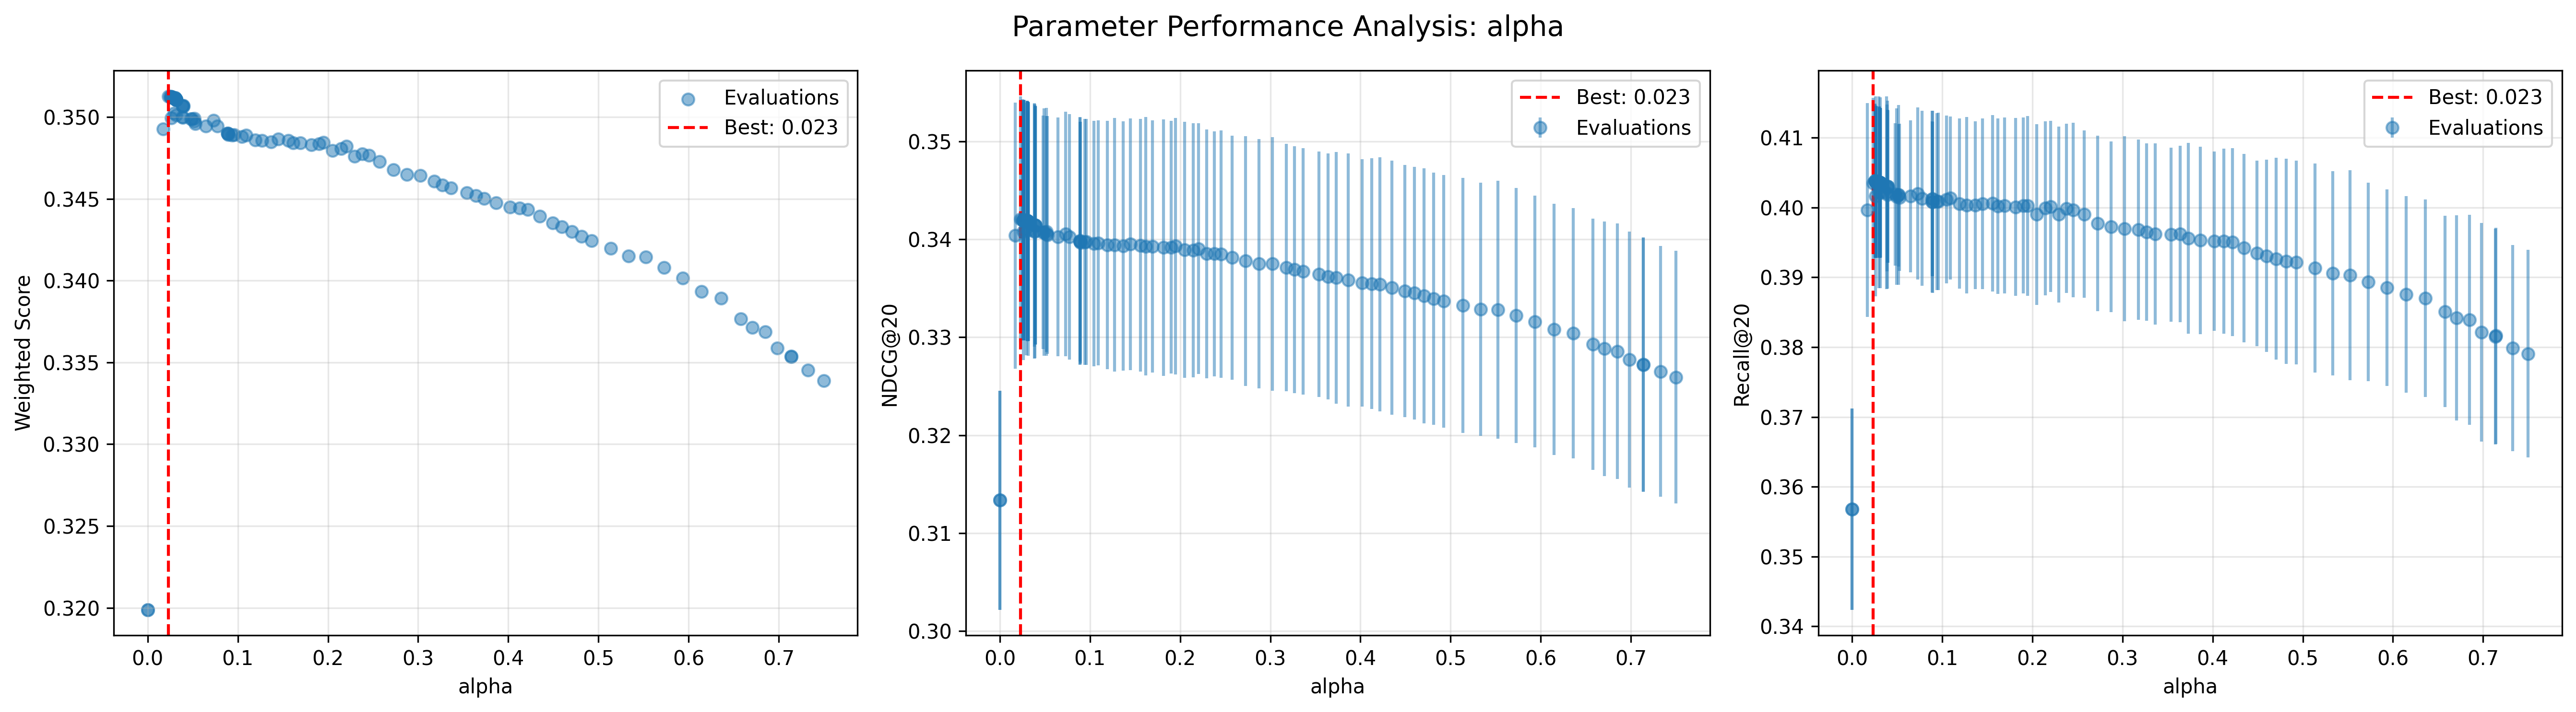
\includegraphics[width=\linewidth]{images/parameter_analysis_alpha.png}
    \caption{Parameter Performance Analysis for Alpha}
    \label{fig:ppr_alpha}
\end{figure}

\begin{figure}[!ht]
    \centering
    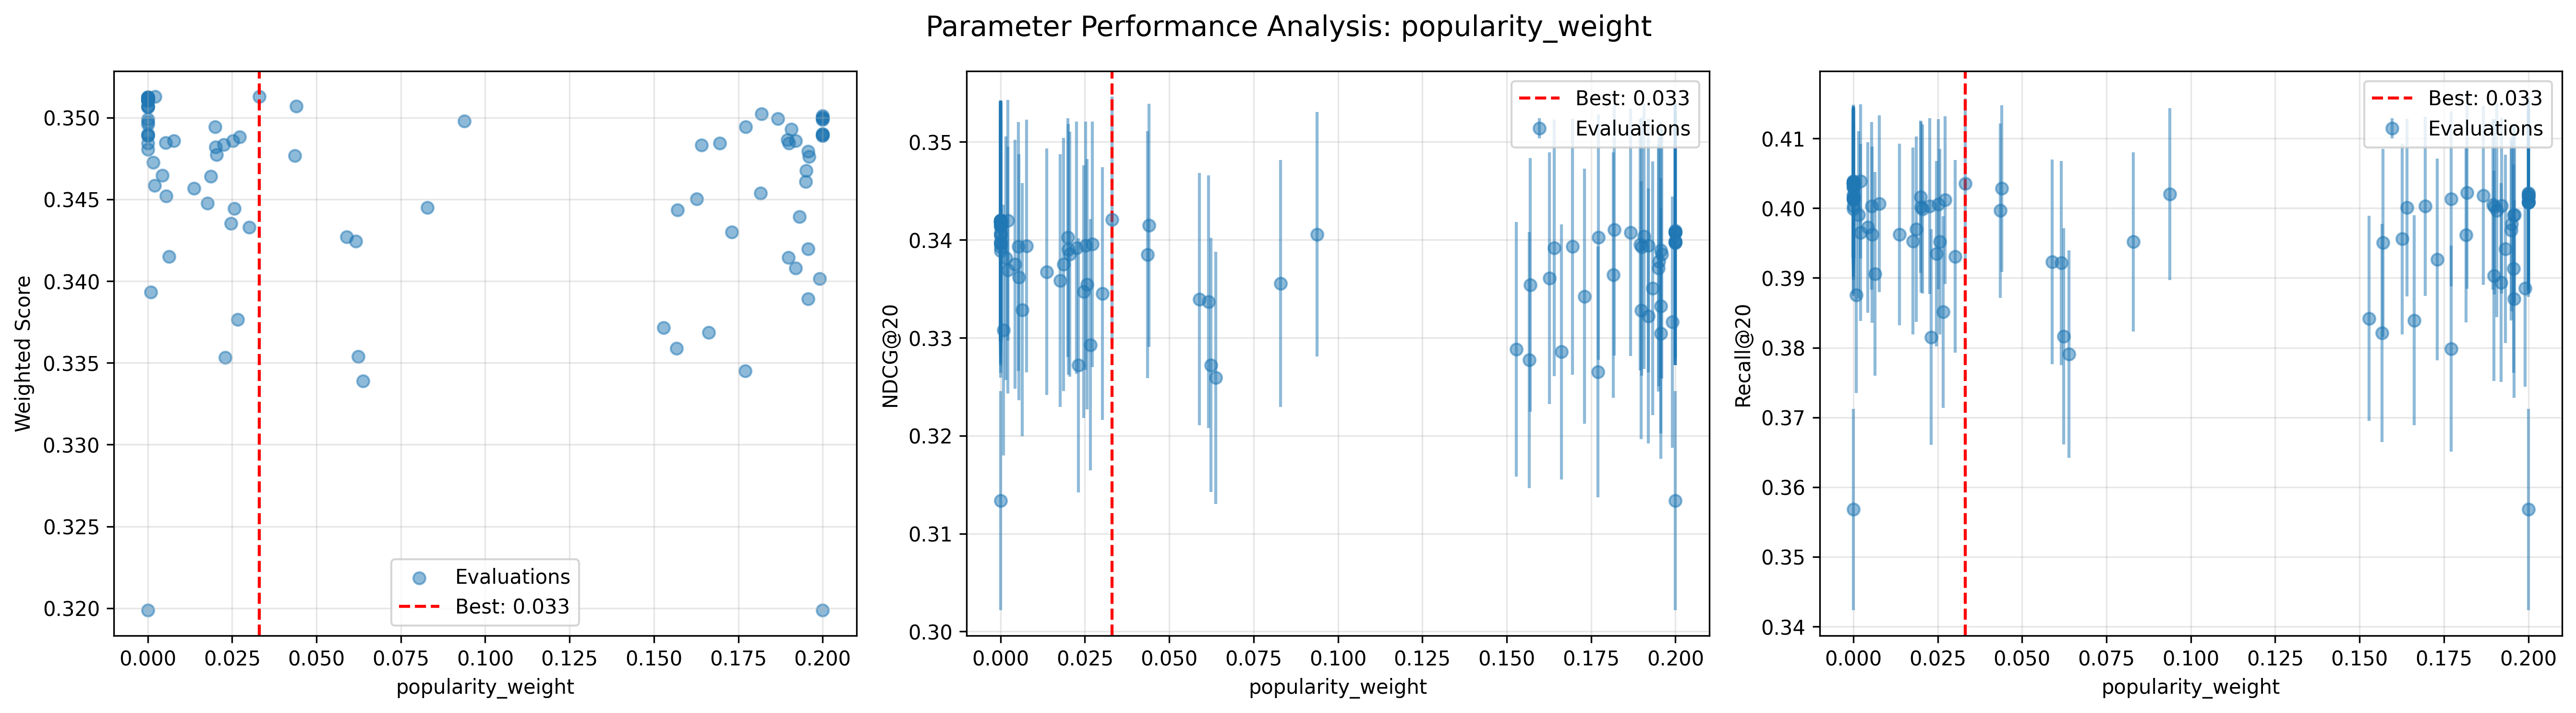
\includegraphics[width=\linewidth]{images/parameter_analysis_popularity_weight.png}
    \caption{Parameter Performance Analysis for Popularity Weight}
    \label{fig:ppr_popularity}
\end{figure}
\begin{figure}[!ht]
    \centering
    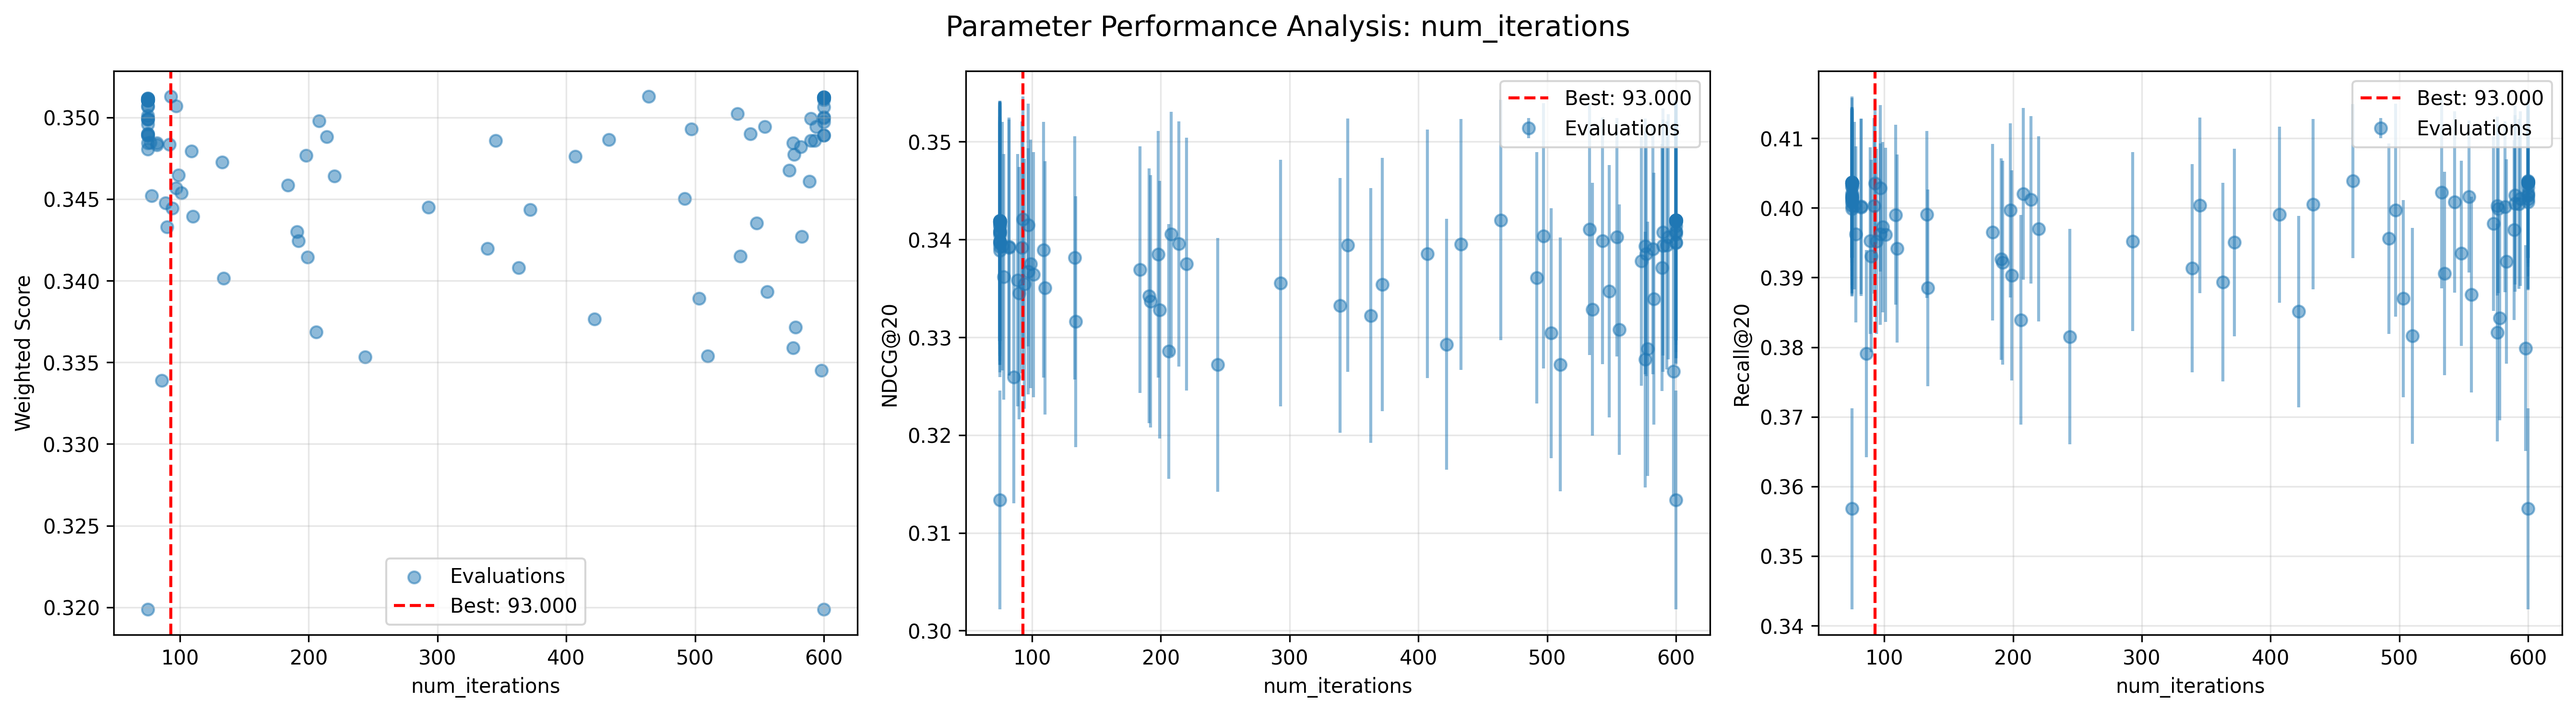
\includegraphics[width=\linewidth]{images/parameter_analysis_num_iterations.png}
    \caption{Parameter Performance Analysis for number of iterations}
    \label{fig:ppr_iterations}
\end{figure}
This demonstrates that the model performs well on the offline dataset, and is also performant in terms of its execution times. The parameter optimization process found a low alpha and popularity weight value to be the best parameter combination, which highlights the importance of user interactions, and minimizes the impact of global popularity metrics.

\subsection{TwoPhase PPR Results}
Table \ref{tab:two_ppr_results} contains the optimized parameters, the offline metrics, and the execution time for the TwoPhase PPR model.  The fact that \(\alpha_2\) is optimized to be 0 indicates that the second phase of the algorithm had no impact on performance and makes the model behave as a base PPR model. The results are similar to the base PPR model, showing that this approach did not provide significant improvements for recommendation quality. A low alpha value is important for the performance of this model, so it is likely that a non-zero alpha would not give a better result. The additional complexity of adding a second phase for recommendation did not have any performance benefits, and was not found to be effective.

\begin{table}[!ht]
    \centering
    \caption{TwoPhase PPR Optimized Parameters and Results}
    \label{tab:two_ppr_results}
    \begin{tabular}{lc}
    \toprule
    \textbf{Parameter} & \textbf{Value} \\
    \midrule
     Alpha1 & 0.041 \\
     Alpha2 & 0.0 \\
     Phase1 K & 148 \\
     Popularity Weight & 0.0\\
     Iterations & 271\\
    Offline NDCG@20 & 0.3453\\
    Offline Recall@20 & 0.4175\\
     Execution Time (s) CPU / GPU & 350 / 40-55 \\
    \bottomrule
    \end{tabular}
\end{table}

The figures \ref{fig:tppr_alpha1}, \ref{fig:tppr_alpha2} and \ref{fig:tppr_stage1k} show the parameter optimization for $\alpha_1$, $\alpha2$ and phase1k respectively. It is clearly shown by the graph that the second alpha is optimized at the lowest value, which essentially removes the second phase. The performance is also relatively consistent, with a low variance as can be seen by the error bars, across a large range of different parameters, especially the phase 1 k parameter, which shows a large region of similar performance. This highlights that the second phase has no impact on the performance of the model.
\begin{figure}[!ht]
    \centering
    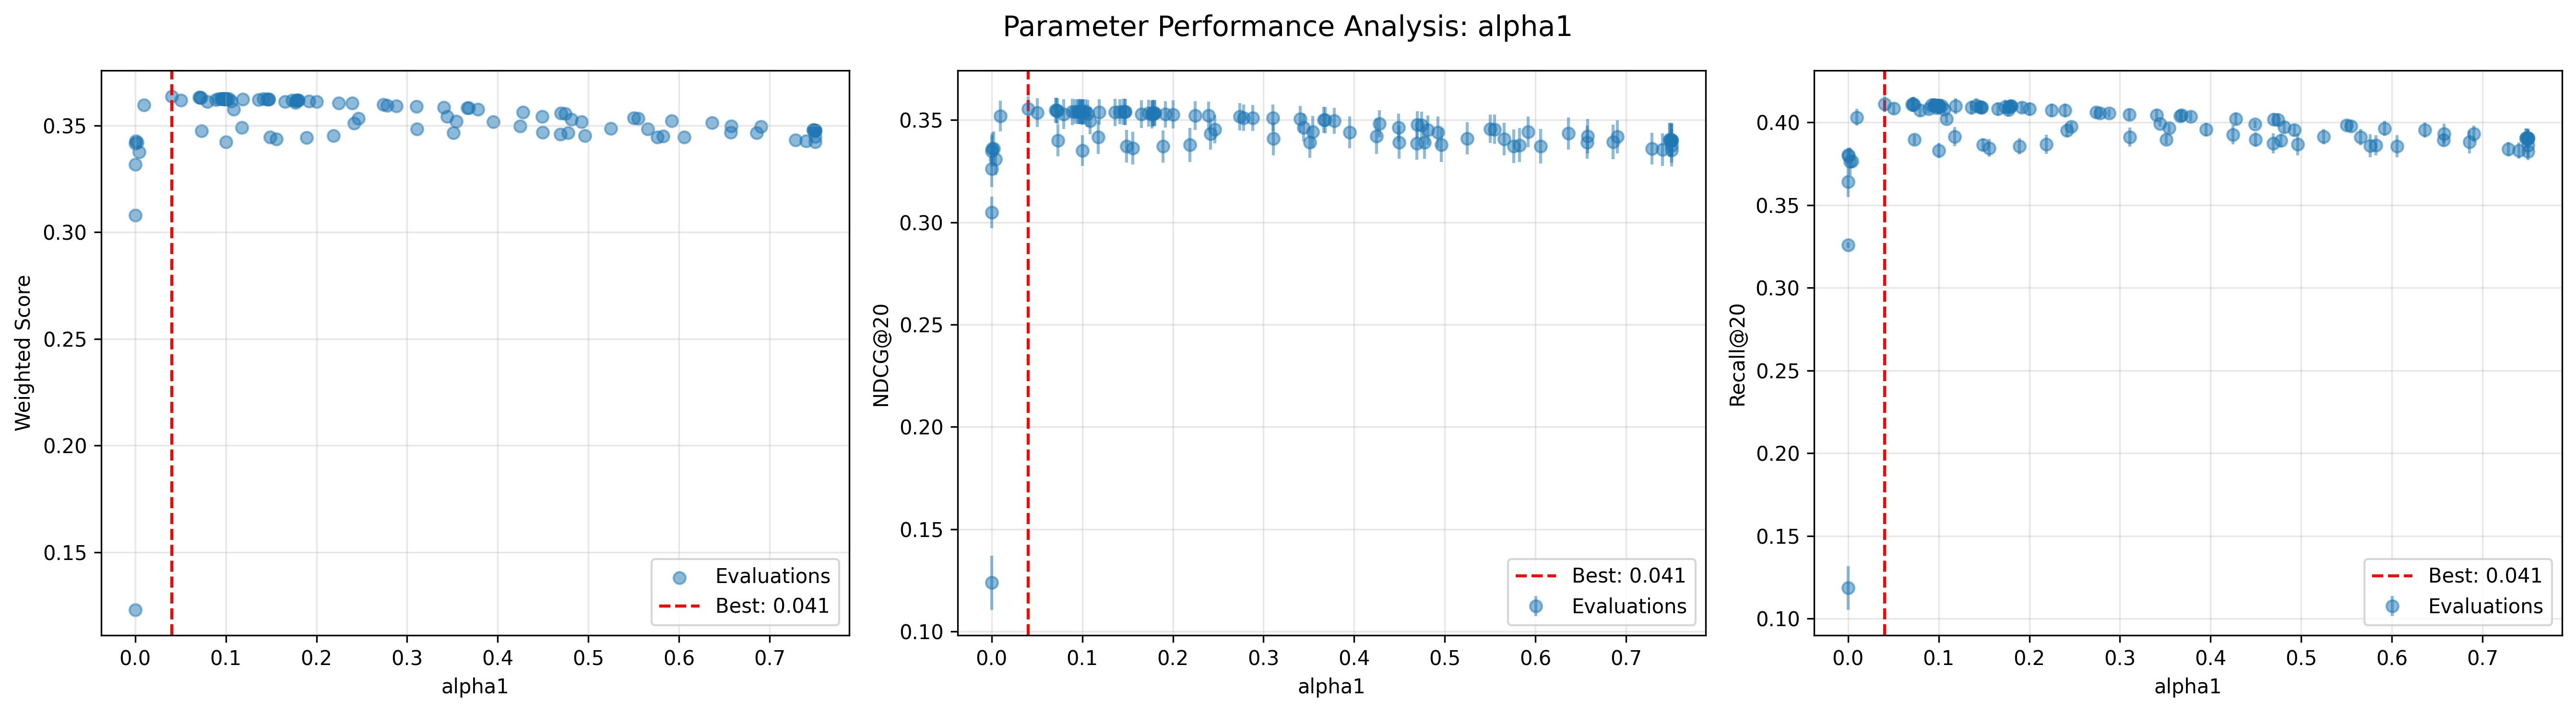
\includegraphics[width=\linewidth]{images/parameter_analysis_alpha1.png}
    \caption{Parameter Performance Analysis for Alpha1}
    \label{fig:tppr_alpha1}
\end{figure}

\begin{figure}[!ht]
    \centering
    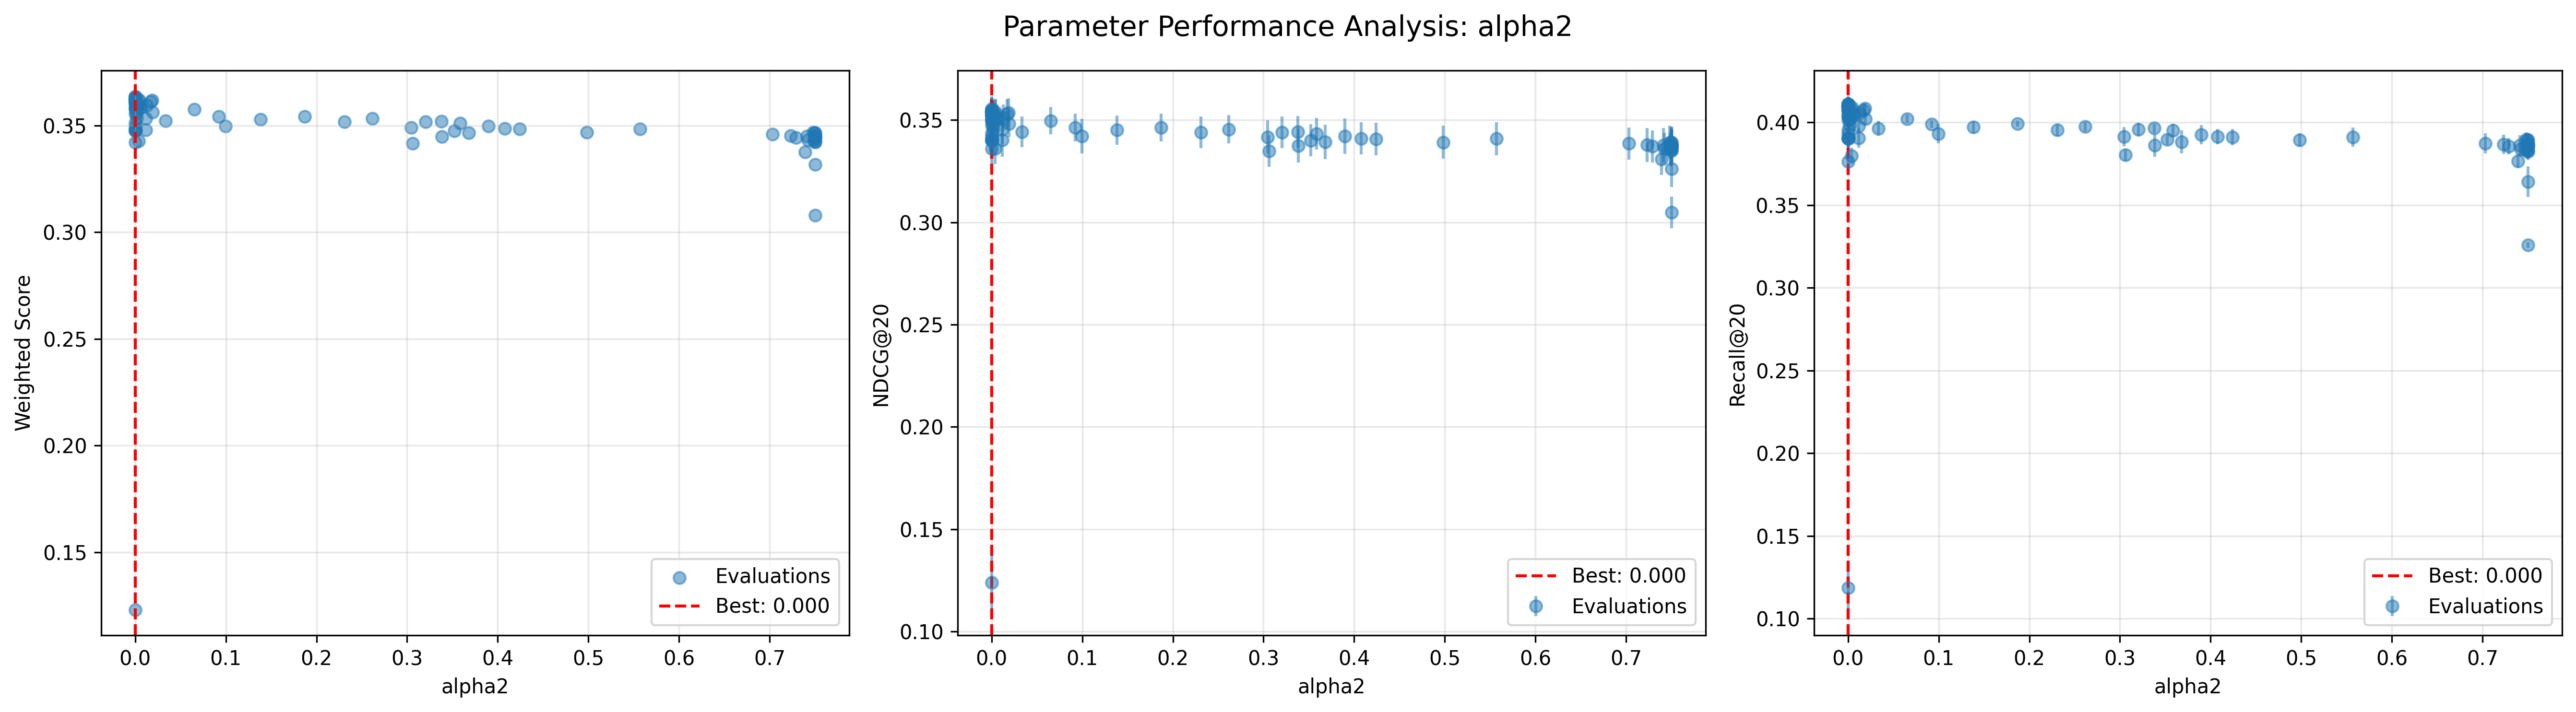
\includegraphics[width=\linewidth]{images/parameter_analysis_alpha2.png}
        \caption{Parameter Performance Analysis for Alpha2}
        \label{fig:tppr_alpha2}
\end{figure}
 \begin{figure}[!ht]
    \centering
    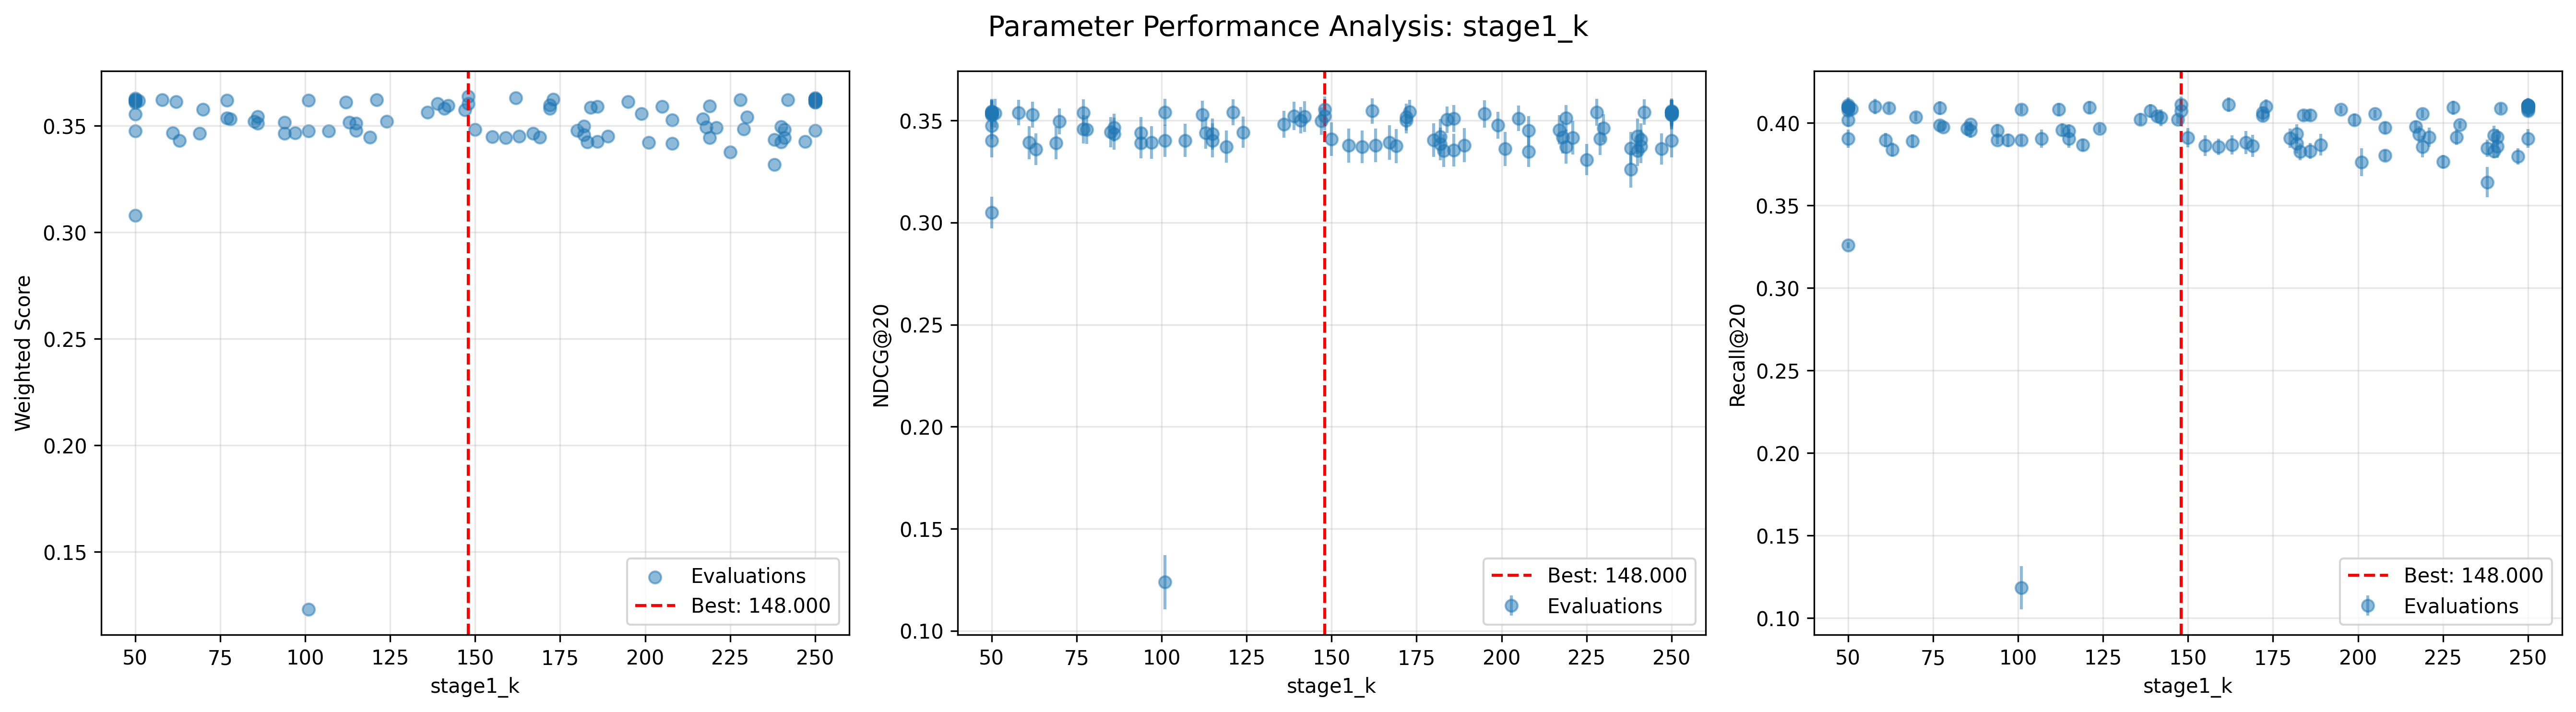
\includegraphics[width=\linewidth]{images/parameter_analysis_stage1_k.png}
    \caption{Parameter Performance Analysis for stage1k}
    \label{fig:tppr_stage1k}
\end{figure}

The execution time is also higher than for the base PPR model, showing that it is not only unable to improve results, it also increases the computational costs. The optimized parameters for this model highlight that it will default to the base implementation, and not capture its key intended benefits.

\subsection{Multi-Alpha PPR Results}
Multi-Alpha PPR achieved a comparable performance to the other PPR variants, as seen in Table \ref{tab:mappr_results}. The optimized weights show that the first alpha, which is close to the optimal value of the single-phase PPR, received all of the weight, while the other alpha values were set to zero. This confirms that a single alpha value is sufficient for high performance, and that adding more alpha values is not beneficial. The higher execution time also means that the method has no real benefits and should be seen as a redundant model.
\begin{table}[!ht]
    \centering
    \caption{Multi-Alpha PPR Optimized Parameters and Results}
        \label{tab:mappr_results}
    \begin{tabular}{lc}
    \toprule
    \textbf{Parameter} & \textbf{Value} \\
    \midrule
     Alphas & [0.023, 0.302, 0.0] \\
     Alpha Weights & [1.0, 0.0, 0.0] \\
     Popularity Weight & 0.0 \\
     Iterations & 106 \\
      Offline NDCG@20 & 0.3450 \\
    Offline Recall@20 & 0.4163 \\
    Execution Time (s) CPU / GPU & 950 / 190 \\
    \bottomrule
    \end{tabular}
\end{table}
Since the method was completely rendered useless by the optimization, the parameter optimization graphs are not included, as there is no significant or useful insights to gain from the plots.

\subsection{Comparative Analysis}
To give a clear view on the performance of all methods, Table \ref{tab:full_comparison} summarizes the online performance of each model.
\begin{table}[!ht]
    \centering
    \caption{Performance Summary of All Algorithms}
    \label{tab:full_comparison}
    \begin{tabular}{@{}lcccc@{}}
    \toprule
    \textbf{Algorithm} & \textbf{SubID} & \textbf{NDCG@20} & \textbf{Recall@20} & \textbf{Time (s)}\\
    \midrule
    Random  & 188908 & 0.002 & 0.003 & 8.32 \\
    Popularity & 188941 & 0.208 & 0.285 & 1.63 \\
    User-kNN & 188910 & 0.208 & 0.285 & 51.30 \\
    Item-kNN & 188503 & 0.320 & 0.352 & 5.65 \\
    PPR & 192184 & 0.318 & 0.379 & 45 \\
    TwoPhasePPR & 192185 & 0.318 & 0.379 & 55 \\
    MultiAlphaPPR & 192183 & 0.319 & 0.380 & 190 \\
    \bottomrule
    \end{tabular}
\end{table}

\begin{figure}[!ht]
    \centering
    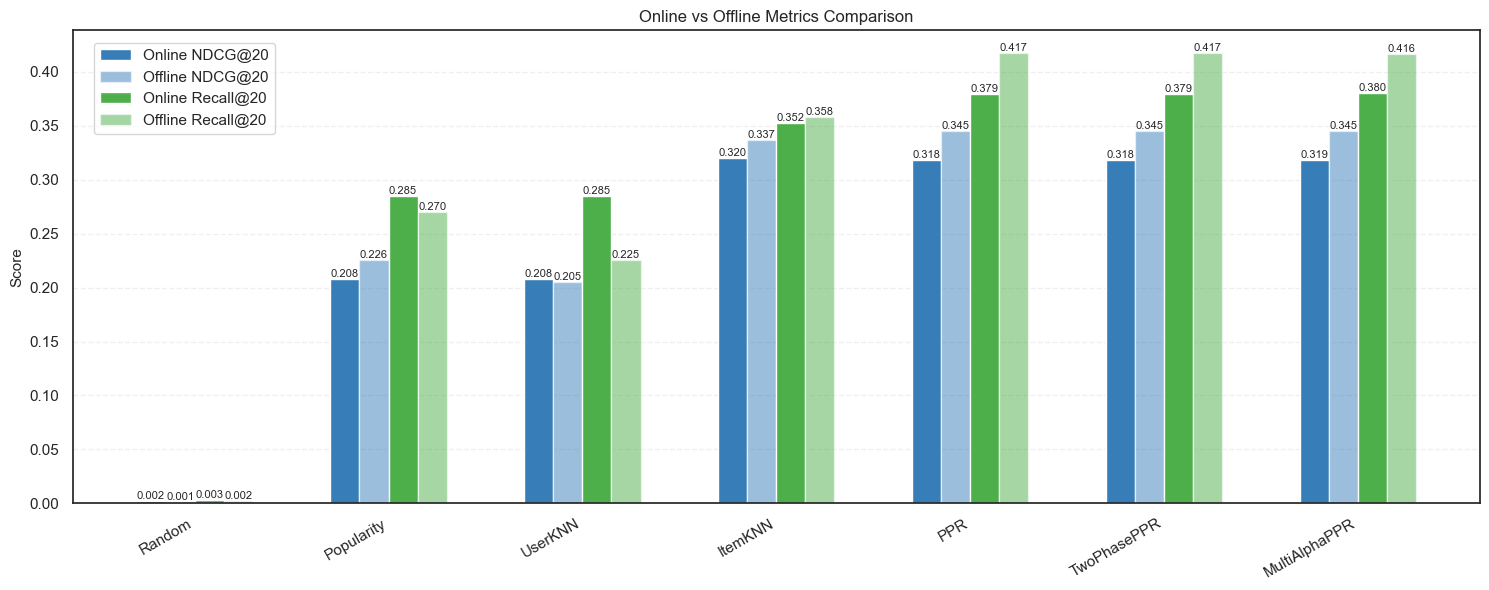
\includegraphics[width=\linewidth]{images/algo_comparison.png}
    \caption{Comparison of the algorithms.}
        \label{fig:algo_comparison}
\end{figure}

The results from the different algorithms show that models that utilize the user item graph and also consider user preferences have a stronger performance than the baselines that just consider global behaviour (like popularity), or simple user or item-based similarities (User-KNN and Item-KNN respectively).

\begin{figure}[!ht]
    \centering
    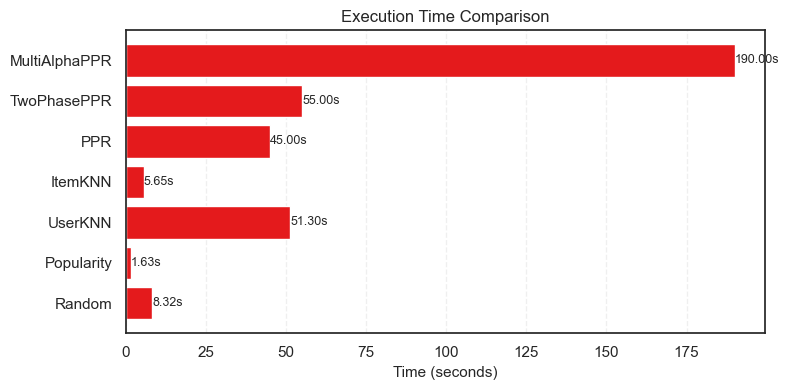
\includegraphics[width=\linewidth]{images/execution_time_comparison.png}
    \caption{Execution time comparison.}
        \label{fig:execution_time_comparison}
\end{figure}

The Item-KNN model achieves a very high level of accuracy, showing that considering item similarities can be a valuable tool for good quality recommendations. The PPR approach shows negligibly worse results on the online metrics than Item-KNN, while also considering personalization. TwoPhase PPR and Multi-Alpha PPR do not give a considerable gain compared to the basic PPR implementation, and also had added complexity that is not justified given their results. This is also observed when looking at the parameters that are optimized by these methods. Multi-Alpha effectively reduces to basic PPR by giving all weight to one alpha value, and TwoPhase PPR makes the second phase useless by optimizing the alpha to a value of 0. In general, all model parameters highlight a preference for personalization, and a low bias towards more exploration in the graph.

\section{Discussion and Analysis}
\subsection{Parameter Analysis and Model Behavior}
Our experiments reveal several key insights about PPR-based recommendation systems. The consistently low optimal alpha values ($\alpha \approx 0.023$) demonstrate that recommendations benefit more from personalization than graph exploration, suggesting that user historical preferences are more predictive of future interests than higher-order relationships. Similarly, the near-zero optimal popularity weight ($w \approx 0.033$) challenges the common assumption that popular items should significantly influence recommendations, instead favoring personalized signals for predicting user preferences.

\subsection{Complexity vs. Performance Trade-offs}
In terms of model complexity, our investigation of PPR variants reveals important insights. The optimization of Two-Phase PPR effectively eliminated its second phase ($\alpha_2 = 0$), indicating that the additional complexity provides no meaningful benefit while increasing computational overhead by approximately 22\%. Similarly, Multi-Alpha PPR's convergence to a single alpha value shows that multiple random walk biases do not capture additional useful information, despite the increased execution time.

\subsection{Performance Comparison}
The comparative analysis between PPR variants and baseline methods yields notable observations. The comparable performance between PPR (NDCG@20 = 0.318) and Item-kNN (NDCG@20 = 0.320) suggests that simple item-based collaborative filtering can be as effective as more complex graph-based approaches in the gaming domain.

\section{Conclusion}
\subsection{Key Findings and Limitations}
Our investigation of graph-based recommendation techniques for Steam revealed that simple approaches achieve comparable performance to complex graph-based methods, PPR variants offer no substantial improvements over the base implementation, and direct user preferences outperform extensive graph exploration.
While hyperparameter tuning was performed on a sampled subset of the data due to computational constraints, we found consistent evidence across multiple experiments that low alpha values lead to better performance. Nevertheless, our approach has several limitations. The evaluation metrics focused primarily on accuracy, leaving potential in unused rich game metadata. Additionally, the strong generalization setting may not fully reflect real-world scenarios where some user history would typically be available.

\subsection{Future Research Directions}
Based on our findings, we propose two main directions for future research. The first involves developing a modified Graph Neural Network approach with item co-occurrence, which constructs a graph based on shared user interactions, captures higher-order relationships between games, and implements graph reduction techniques.

The second direction focuses on hybrid content-based approaches. Integrating content-based features with PPR could enhance recommendation quality by incorporating game attributes, leveraging both interaction patterns and content similarity, and addressing cold-start problems for new games.

\section*{Acknowledgments}
Large language models were used in the writing and editing of portions of this paper.


\nocite{*}
\bibliographystyle{IEEEtran}
\bibliography{references}

\end{document}